% Options for packages loaded elsewhere
\PassOptionsToPackage{unicode}{hyperref}
\PassOptionsToPackage{hyphens}{url}
%
\documentclass[
]{article}
\usepackage{amsmath,amssymb}
\usepackage{lmodern}
\usepackage{iftex}
\ifPDFTeX
  \usepackage[T1]{fontenc}
  \usepackage[utf8]{inputenc}
  \usepackage{textcomp} % provide euro and other symbols
\else % if luatex or xetex
  \usepackage{unicode-math}
  \defaultfontfeatures{Scale=MatchLowercase}
  \defaultfontfeatures[\rmfamily]{Ligatures=TeX,Scale=1}
\fi
% Use upquote if available, for straight quotes in verbatim environments
\IfFileExists{upquote.sty}{\usepackage{upquote}}{}
\IfFileExists{microtype.sty}{% use microtype if available
  \usepackage[]{microtype}
  \UseMicrotypeSet[protrusion]{basicmath} % disable protrusion for tt fonts
}{}
\makeatletter
\@ifundefined{KOMAClassName}{% if non-KOMA class
  \IfFileExists{parskip.sty}{%
    \usepackage{parskip}
  }{% else
    \setlength{\parindent}{0pt}
    \setlength{\parskip}{6pt plus 2pt minus 1pt}}
}{% if KOMA class
  \KOMAoptions{parskip=half}}
\makeatother
\usepackage{xcolor}
\usepackage[margin=1in]{geometry}
\usepackage{graphicx}
\makeatletter
\def\maxwidth{\ifdim\Gin@nat@width>\linewidth\linewidth\else\Gin@nat@width\fi}
\def\maxheight{\ifdim\Gin@nat@height>\textheight\textheight\else\Gin@nat@height\fi}
\makeatother
% Scale images if necessary, so that they will not overflow the page
% margins by default, and it is still possible to overwrite the defaults
% using explicit options in \includegraphics[width, height, ...]{}
\setkeys{Gin}{width=\maxwidth,height=\maxheight,keepaspectratio}
% Set default figure placement to htbp
\makeatletter
\def\fps@figure{htbp}
\makeatother
\setlength{\emergencystretch}{3em} % prevent overfull lines
\providecommand{\tightlist}{%
  \setlength{\itemsep}{0pt}\setlength{\parskip}{0pt}}
\setcounter{secnumdepth}{-\maxdimen} % remove section numbering
\newlength{\cslhangindent}
\setlength{\cslhangindent}{1.5em}
\newlength{\csllabelwidth}
\setlength{\csllabelwidth}{3em}
\newlength{\cslentryspacingunit} % times entry-spacing
\setlength{\cslentryspacingunit}{\parskip}
\newenvironment{CSLReferences}[2] % #1 hanging-ident, #2 entry spacing
 {% don't indent paragraphs
  \setlength{\parindent}{0pt}
  % turn on hanging indent if param 1 is 1
  \ifodd #1
  \let\oldpar\par
  \def\par{\hangindent=\cslhangindent\oldpar}
  \fi
  % set entry spacing
  \setlength{\parskip}{#2\cslentryspacingunit}
 }%
 {}
\usepackage{calc}
\newcommand{\CSLBlock}[1]{#1\hfill\break}
\newcommand{\CSLLeftMargin}[1]{\parbox[t]{\csllabelwidth}{#1}}
\newcommand{\CSLRightInline}[1]{\parbox[t]{\linewidth - \csllabelwidth}{#1}\break}
\newcommand{\CSLIndent}[1]{\hspace{\cslhangindent}#1}
\ifLuaTeX
  \usepackage{selnolig}  % disable illegal ligatures
\fi
\IfFileExists{bookmark.sty}{\usepackage{bookmark}}{\usepackage{hyperref}}
\IfFileExists{xurl.sty}{\usepackage{xurl}}{} % add URL line breaks if available
\urlstyle{same} % disable monospaced font for URLs
\hypersetup{
  pdftitle={JSE Delistings and Stock Prices},
  pdfauthor={Elias Muchineripi Mashayamombe},
  hidelinks,
  pdfcreator={LaTeX via pandoc}}

\title{JSE Delistings and Stock Prices}
\author{Elias Muchineripi Mashayamombe}
\date{2023-02-02}

\begin{document}
\maketitle

\newpage

\hypertarget{firms-listed-in-study}{%
\section{Firms Listed in Study}\label{firms-listed-in-study}}

\begin{enumerate}
\def\labelenumi{\arabic{enumi}.}
\tightlist
\item
  ``WHL'': WHK Group Limited.
\item
  ``MTN'': MTN Group Limited.
\item
  ``SOL'': Sasol Limited.
\item
  ``SHP'': Shoprite Holdings Limited.
\item
  ``BVT'': Bavaria Industries Group Limited.
\item
  ``IMP'': Impala Platinum Holdings Limited.
\item
  ``HAR'': Harmony Gold Mining Company Limited.
\item
  ``DSY'': Distell Group Limited
\item
  ``SNT'': Santova Logistics Limited
\item
  ``AIP'': Afriplex (Pty) Ltd.
\item
  ``RMB'': Rand Merchant Bank (a division of FirstRand Bank Limited).
\item
  ``STX'': Satrix Limited.
\item
  ``ADR'': Adcock Ingram Holdings Limited.
\item
  ``SBK'': Standard Bank Group Limited.
\item
  ``CFR'': Clinix Health Group Limited.
\item
  ``INL'': Invicta Holdings Limited.
\item
  ``TFG'': The Foschini Group Limited.
\item
  ``PSG'': PSG Group Limited.
\item
  ``KBO'': Kalon Venture Capital Proprietary Limited.
\end{enumerate}

\newpage

\hypertarget{introduction}{%
\section{Introduction}\label{introduction}}

Following COVID19, concerns where raised over the number of delsitings
on the Johannesburg Stock Exchange (JSE). With market commentators
already discussing the `slow death' of the JSE, it's CEO had to jump to
it's defense. After taking note of the criticism, Fourie described South
Africans congenitally negative and went on to plead with all
stakeholders to put out positive sentiments that would ultimately crowd
in investments.

The figure below shows the number of listings and delsitings from 1992
to 2021.

\begin{figure}
\centering
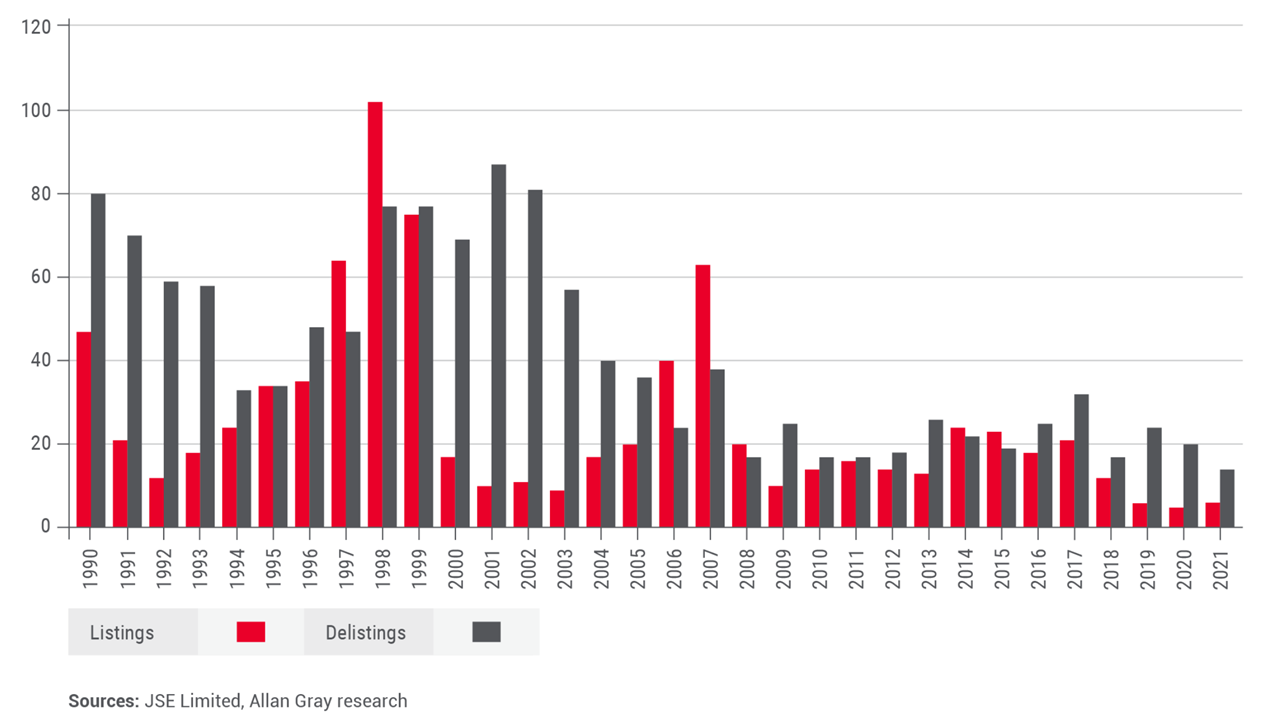
\includegraphics{delist.png}
\caption{Number of New Listings and Delistings}
\end{figure}

In light of a clear increase in the number of delisitings, we
investigate how share prices have moved and build machine learning model
that try and predict the stock prices of 20 randomly selcted pcompanies
still listed on the JSE.

\hypertarget{literature-reveiw}{%
\section{Literature Reveiw}\label{literature-reveiw}}

(Cassim 2000) provide a historical background of the JSE and its
evolution from its inception in 1887 to its current form as a modern
stock exchange. Cassim and Herbst provide an overview of the JSE's
governance structure, its role in the South African economy, and the
types of securities traded on the JSE. This study particularly
highlighted the importance of the JSE as an indicator of the health of
the South African economy and as a source of capital for companies in
South Africa making it an institution of critical importance. In a
similar study Addison and A. Odendaal, (Addison S. 2008), provided a
comprehensive overview of the JSE's history, starting from its
establishment in 1887 to its development in the 20th century. Trace the
evolution of the JSE and its role in the South African economy, focusing
on the exchange's role in supporting the growth of new industries and
providing capital for businesses, the article examined the JSE's
innovations and how they have contributed to its growth and development.
They discussed the introduction of new technologies, such as electronic
trading systems, and the creation of new financial products, such as
derivatives, which have enabled the JSE to compete with other leading
stock exchanges in the world. The article highlighted the challenges
faced by the JSE, including political and economic turmoil, and how the
exchange has adapted to overcome these challenges. The authors concluded
that the JSE has been a leading player in the financial industry,
consistently adapting to changes in the economy and technology to
maintain its position as one of the leading stock exchanges in Africa.
(McDonald 2006), studied the Johannesburg Stock Exchange (JSE) and its
listings in the post-apartheid era. The study provided a historical
background of the JSE, its role in the South African economy, and its
evolution in the post-apartheid era. With an overview of the JSE's
governance structure, its listing requirements, and the types of
securities traded on the JSE, the article consequently highlighted the
impact of the post-apartheid political and economic reforms on the JSE
and its listings. The increased foreign investment in the JSE, and the
growth of new industries and companies listed on the exchange were
discussed as well as the challenges facing the JSE and its listings,
including increased competition from other stock exchanges and the need
for further economic and political reforms. (McDonald 2006), argued that
the JSE had the potential to play a significant role in the growth and
development of the South African economy, and that continued reforms
where necessary to ensure its continued success. (Al-Hawari 2010),
demonstrated that delisting from the Johannesburg Stock Exchange can
have significant impact on shareholder wealth and stock prices. They
provided evidence on the phenomenon of delisting in emerging markets,
specifically the Johannesburg Stock Exchange (JSE) and examined the
reasons for delisting and the impact of delisting on firm value. The
authors used a sample of delisted firms from the JSE for the period from
1997 to 2007. The results of the study show that the main reasons for
delisting from the JSE are financial distress, management decisions, and
mergers and acquisitions. The results also indicate that delisted firms
experience a decline in firm value, and that the decline in firm value
is more pronounced for firms that delist due to financial distress. The
results of the study are relevant for investors, regulators, and policy
makers in emerging markets. Roy, et al, (Roy 2010), study the liquidity
and market quality of the Johannesburg Stock Exchange (JSE). They
analyzed the liquidity and market quality of the JSE over a period of
ten years (1997-2006) and compared the results with other major stock
exchanges around the world. The authors find that the liquidity of the
JSE is generally good, but there is a considerable amount of illiquidity
in the market, particularly in the smaller stocks. They also find that
the market quality of the JSE is lower than that of other major stock
exchanges, due to a high degree of market manipulation, and the absence
of regulations to prevent insider trading and other forms of market
abuse. The authors suggested that the JSE should implement measures to
improve market quality, such as increasing transparency, and
strengthening regulations to prevent market abuse. They also recommend
that the JSE should invest in new technologies, such as electronic
trading systems, to improve the efficiency and competitiveness of the
exchange.

(Chutta 2015), The authors investigate the causes and consequences of
delistings from the Johannesburg Stock Exchange (JSE). The study uses a
sample of 50 companies that delisted from the JSE between 2006 and 2011
and compares them to a control sample of firms that remained listed
during the same period. The results suggest that delistings are
associated with lower liquidity, higher leverage, and lower
profitability compared to firms that remain listed. The authors conclude
that delisting is a negative outcome for both firms and investors and
that regulators should consider policies that support the continued
listing of firms on stock exchanges.

According to Hugo and Chen, (Hugo 2017), the determinants of delisting
from the Johannesburg Stock Exchange include various financial and
non-financial factors such as profitability, liquidity, and size. The
study examines the factors that lead firms to delist from the
Johannesburg Stock Exchange (JSE). The authors use a panel data set of
listed firms on the JSE over a period of 21 years to investigate the
determinants of delistings. They find that firm-specific factors such as
financial performance, size, and age, as well as market-wide factors
such as macroeconomic conditions, play a significant role in the
likelihood of delisting. The authors conclude that their findings
provide important insights for policymakers and regulators looking to
improve the functioning of stock exchanges in emerging markets. (Ntusi
2019), focus on the impact of delistings on shareholder wealth in the
Johannesburg Stock Exchange (JSE). The authors used event study
methodology to examine the impact of delistings announcements on
shareholder wealth around the event. The results suggest that delistings
announcements have a negative impact on shareholder wealth, and the
magnitude of the effect is higher for smaller firms. The findings have
implications for regulators and policymakers, suggesting the need for
increased monitoring of delistings to protect the interests of small
shareholders.

(Magagula 2020), employed a sample of 25 firms delisted from the JSE
between 2013 and 2016 and uses event study methodology to examine the
stock prices of these firms both prior to and after delisting. The
results suggest that delisting has a negative impact on stock prices,
and the magnitude of this effect is influenced by the reasons for
delisting and the characteristics of the firms involved. The authors
conclude that regulators should be mindful of the negative effects of
delisting and work to ensure that such events are managed in a manner
that minimizes harm to stakeholders.

\hypertarget{including-plots}{%
\subsection{Including Plots}\label{including-plots}}

You can also embed plots, for example:

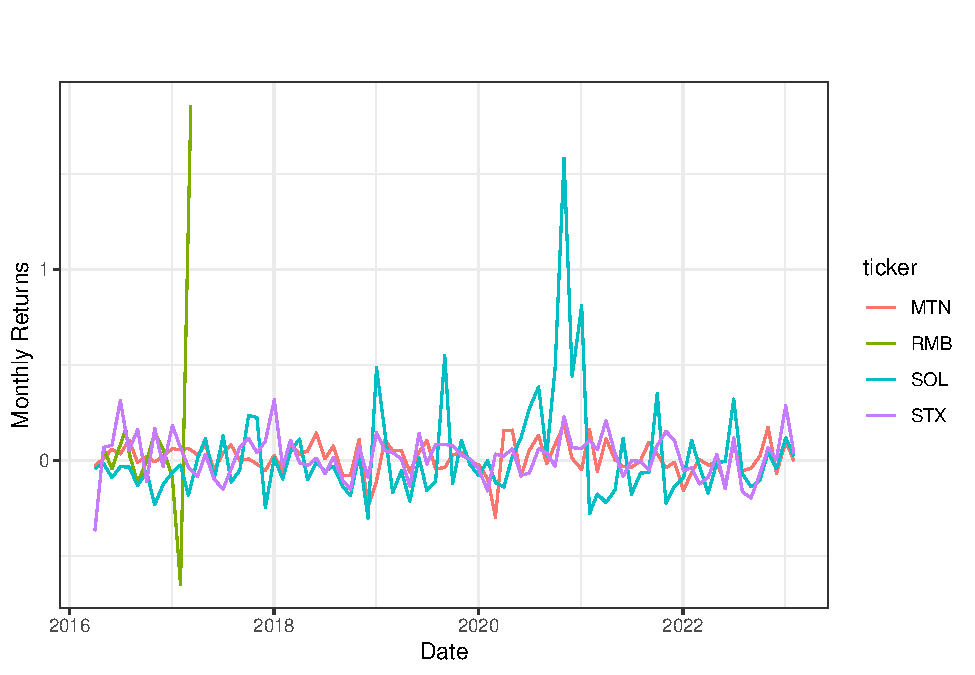
\includegraphics{JSE_Stocks_files/figure-latex/returns_plot-1.pdf}

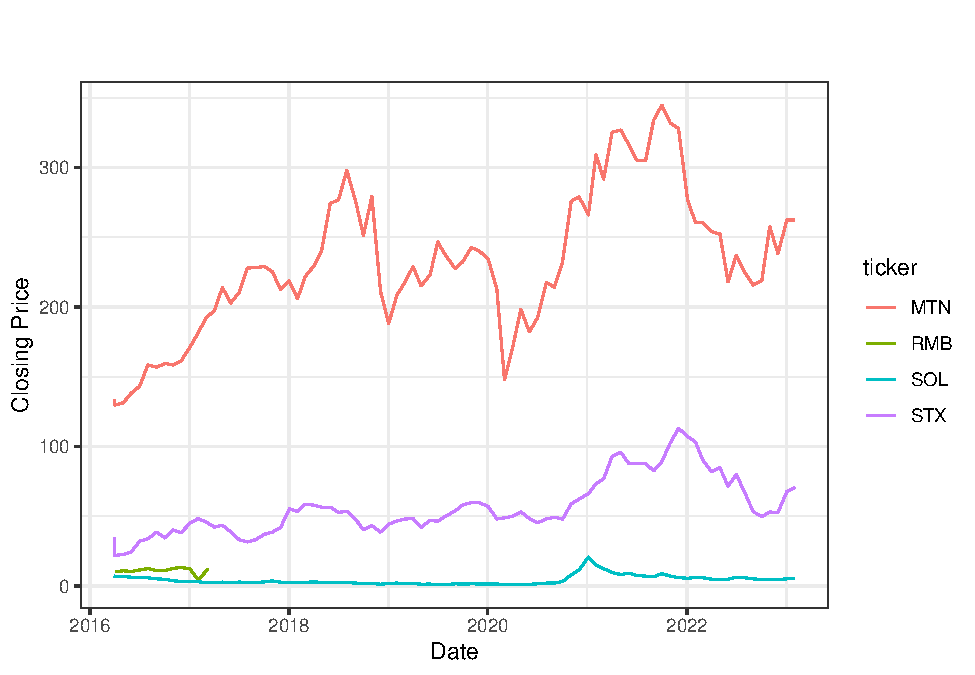
\includegraphics{JSE_Stocks_files/figure-latex/prices_plot-1.pdf}

\hypertarget{pre-processing-the-data}{%
\section{Pre-processing the Data}\label{pre-processing-the-data}}

In our data pre-processing, we opt to get the data for only the
``price.close'' column. Using the caTools package we split the data set
into our training set and the test set.

\hypertarget{evaluating-the-model}{%
\section{Evaluating the Model}\label{evaluating-the-model}}

Calculate the mean absolute error (MAE)

\hypertarget{concluding-remarks}{%
\section{Concluding Remarks}\label{concluding-remarks}}

\hypertarget{references}{%
\section{References}\label{references}}

\bibliography{references.bib}

\hypertarget{refs}{}
\begin{CSLReferences}{1}{0}
\leavevmode\vadjust pre{\hypertarget{ref-addison2008hist}{}}%
Addison S., Odendaal A. 2008. {``The Johannesburg Stock Exchange: A
History of Innovation.''} \emph{South African Journal of Economic
History} 23 (1): 1--19.

\leavevmode\vadjust pre{\hypertarget{ref-alhawari2010delisting}{}}%
Al-Hawari, Papke, M. E. 2010. {``Delisting in Emerging Markets: Evidence
from the Johannesburg Stock Exchange.''} \emph{Journal of Emerging
Market Finance} 9 (3): 299--323.

\leavevmode\vadjust pre{\hypertarget{ref-cassim2000jse}{}}%
Cassim, \& Herbst, M. L. 2000. {``The Johannesburg Stock Exchange: An
Overview.''} \emph{Journal of African Business} 1 (1): 1--18.

\leavevmode\vadjust pre{\hypertarget{ref-chutta2015delist}{}}%
Chutta, Dimitropoulos, K. S. 2015. {``Delistings from the Johannesburg
Stock Exchange: Causes, Characteristics and Consequences.''}
\emph{Journal of African Business} 16 (4): 333--54.

\leavevmode\vadjust pre{\hypertarget{ref-hugo2017determ}{}}%
Hugo, \& Chen, D. L. 2017. {``The Determinants of Delistings from the
Johannesburg Stock Exchange.''} \emph{Journal of Financial Regulation
and Compliance} 25 (4): 338--58.

\leavevmode\vadjust pre{\hypertarget{ref-magagula2020conseq}{}}%
Magagula, \& Moemi, N. I. 2020. {``The Consequences of Delisting on
Stock Prices: Evidence from the Johannesburg Stock Exchange.''}
\emph{African Journal of Accounting, Auditing and Finance} 9 (1):
51--63.

\leavevmode\vadjust pre{\hypertarget{ref-mcdonald2006post}{}}%
McDonald, D. G. 2006. {``Post-Apartheid South Africa: A Study of the
Johannesburg Stock Exchange and Its Listings.''} \emph{Journal of
Transnational Management} 11 (3): 175--95.

\leavevmode\vadjust pre{\hypertarget{ref-ntusi2019impact}{}}%
Ntusi, \& Moemi, C. Z. 2019. {``The Impact of Delistings on Shareholder
Wealth: Evidence from the Johannesburg Stock Exchange.''} \emph{Journal
of Applied Economics and Business Research} 8 (4): 249--66.

\leavevmode\vadjust pre{\hypertarget{ref-roy2010liq}{}}%
Roy, Longstaff, T. K. 2010. {``Liquidity and Market Quality in the
Johannesburg Stock Exchange.''} \emph{Journal of Financial
Intermediation} 19 (2): 246--65.

\end{CSLReferences}

\end{document}
